\chapter{Related Work}
In this chapter, we first review a set of work that aims to enable touch interaction on everyday surfaces and objects. Then we dive deeper into prior work in the field of capacitive sensing closely related to \textit{FlexTouch} to better position our work in the related literature.

\section{Touch Interaction on Everyday Surfaces and Objects}
Researchers have explored various methods and techniques to enable interactive interfaces on everyday surfaces and objects. One popular method to enable touch interactions, as shown in Fig ~\ref{fig:cv-large-scale-interaction} is by projecting 2D user interfaces onto a surface and then recognize user interaction via computer vision technique ~\cite{pinhanez2001everywhere, Fails-2002-Light-Widgets, Wilson-2010-Light-Space, Xiao-WorldKit}. For example, \textit{WorldKit} system makes use of a paired projector and a depth camera to capture user's touch-based interaction on surfaces, enabling people to quickly instantiate any shapes of interface they like. To achieve this, the system also requires preconfiguration of functionality of different locations on the surface. Apparently, these solutions can support large-scale interactions which are suitable for fixed infrastructure. However, its power consumption and form factor still make it hard to fit into everyday mobile scenarios. Furthermore, the cost of the toolkit as well as the difficulty of setup also makes it far way from being popularized to the industry.

\begin{figure}[ht]
    \centering
	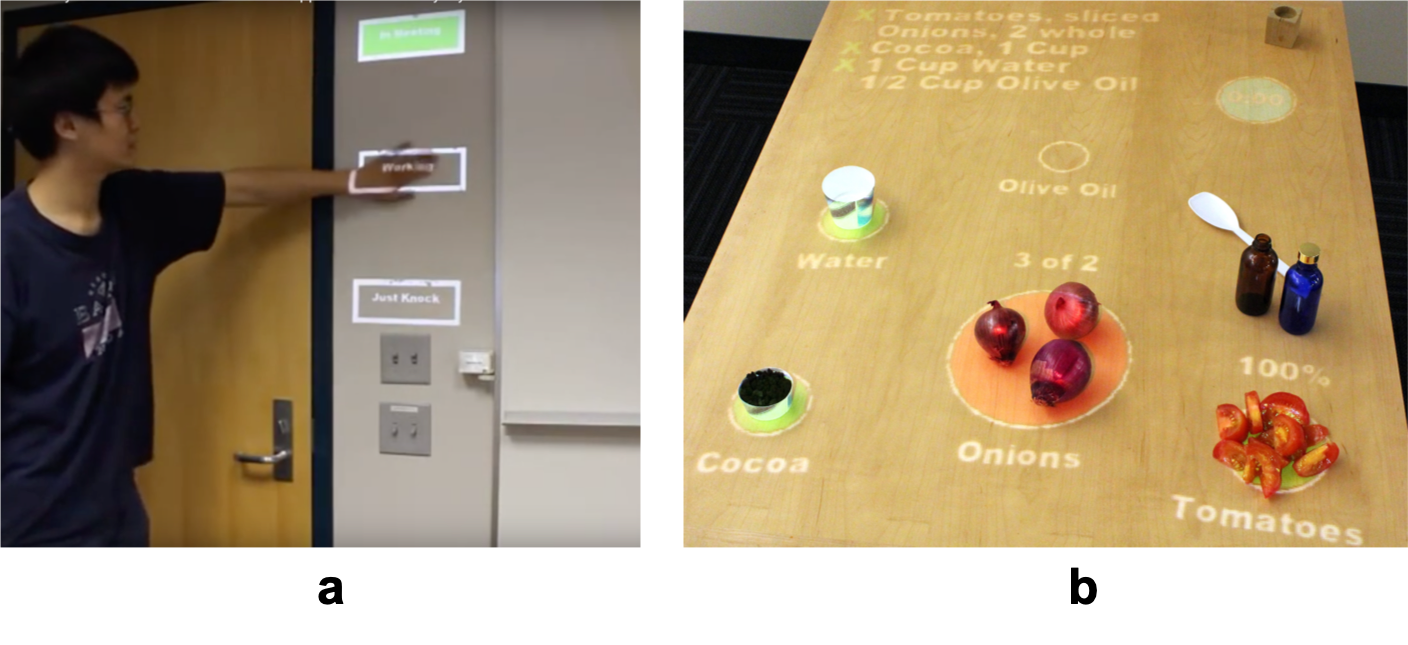
\includegraphics[width=0.95\columnwidth]{figures/cv-large-scale-sensing.png}
	\setlength{\belowcaptionskip}{-6pt}
    \caption{Example applications of vision-based large-scale interaction: a) notification message application. b) Kitchen application.}
    \label{fig:cv-large-scale-interaction}
\end{figure}

Touch interaction can also be supported by acoustic sensing.  Ono's work is based on the difference of resonate properties of different objects ~\cite{Ono-Touch-and-Activate}. As illustrated in Fig \ref{fig:acoustic-sensing}, by attaching a viabration speaker and a piezo-electric microphone, the system collects and amplify the vibration data and transmit it into a computational device. Then, by train a supervised pattern recognition model for recognizing different acoustic wave patterns, it is able to distinguish various touch events. Researchers have also explored recognizing a discrete set of touch events on everyday objects such as windows ~\cite{Paradiso-2002-Window}, desktops, and other surfaces ~\cite{Harrison-2008-Scratch-iput}. However, these approaches can only be applied towards a small set of touch inputs like tapping or scratching on various materials. Last but not least, these approaches cannot live without dedicated sensing platforms to collect and transmit acoustic data from objects, which adds too much complexity to existing objects.

\begin{figure}[ht]
    \centering
	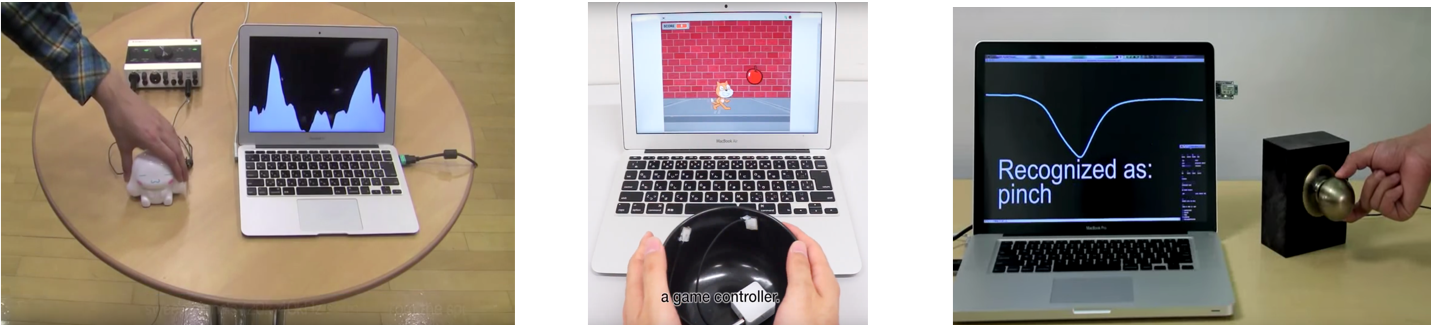
\includegraphics[width=0.88\columnwidth]{figures/acoustic-sensing.png}
	\setlength{\belowcaptionskip}{-6pt}
    \caption{Touch and Activate: Adding interactivity of existing objects using active acoustic sensing}
    \label{fig:acoustic-sensing}
\end{figure}

Another popular method is electromagnetic sensing. \textit{SmartSkin} enabled multi-touch interaction on surfaces using a mesh-shaped capacitive sensor grid ~\cite{Rekimoto-SmartSkin}. They make use of a capacitive sensor grid with size of 32 \times 24 to detect touch events on a large-scale surface. 
\begin{figure}[ht]
    \centering
	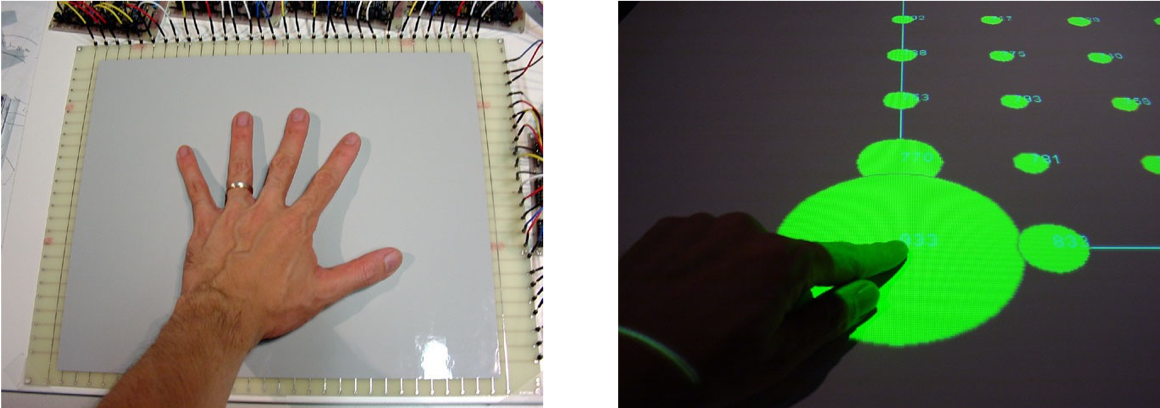
\includegraphics[width=0.88\columnwidth]{figures/smartskin.png}
	\setlength{\belowcaptionskip}{-6pt}
    \caption{\textit{SmartSkin} is embedded with dense capacitive sensors to achieve accurate touch sensing on flat surface.}
    \label{fig:smartskin}
\end{figure}

\textit{Electrick} ~\cite{Zhang-Electrick} and \textit{Pulp Nonfiction} ~\cite{Zhang-pulp} enabled touch input on everyday surfaces and objects using Electric Field Tomography (EIT) with coated conductive materials on everyday surfaces and objects. As shown in Fig ~\ref{fig:electrick}, by sensing the voltage difference between paired electrodes before and after touch, \textit{Electrick} can accurately locates user's touch position as well as measuring the pressure of touch event. 

\begin{figure}[ht]
    \centering
	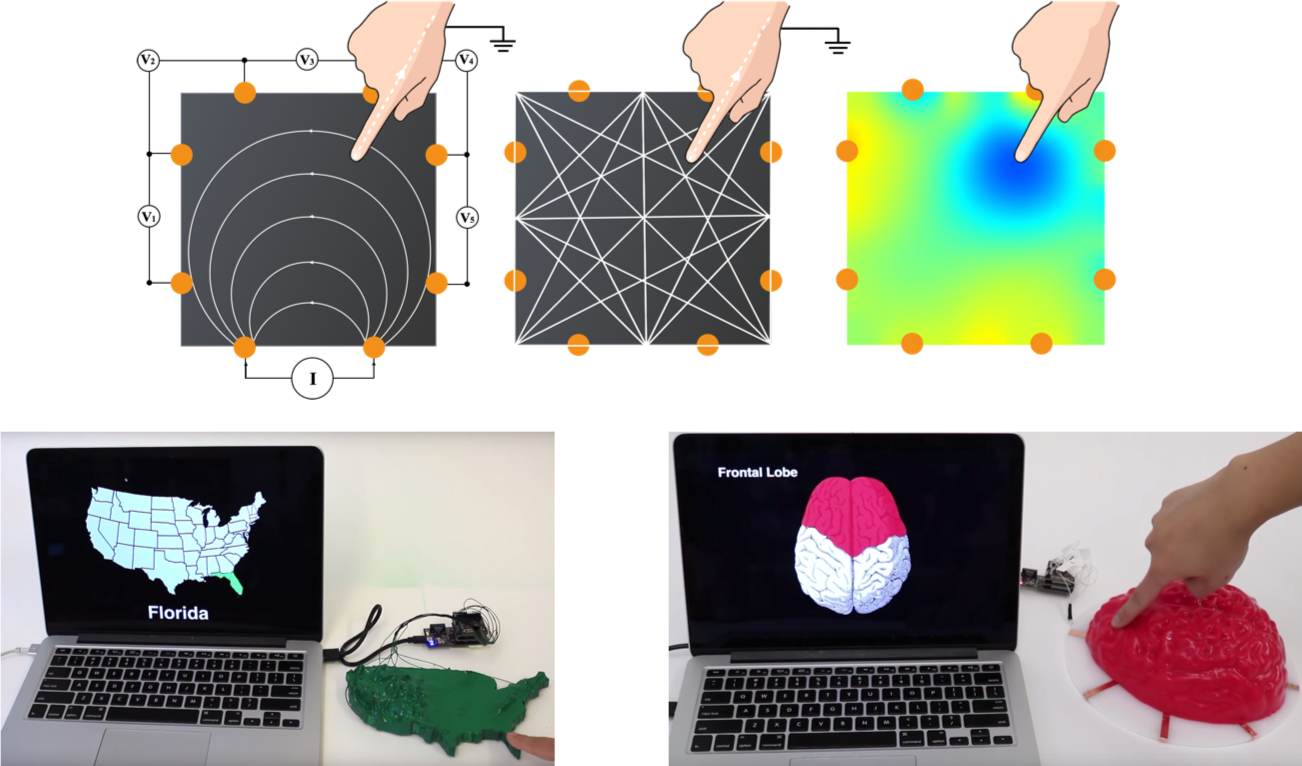
\includegraphics[width=0.88\columnwidth]{figures/electrick.png}
	\setlength{\belowcaptionskip}{-6pt}
    \caption{\textit{Electrick}: Enabling low-cost touch sensing on any shapes of surfaces by using electric field tomography}
    \label{fig:electrick}
\end{figure}

\textit{Touche} ~\cite{Sato-Touche} enhances touch interface on the human body or everyday objects by measuring the electrical profiles with a frequency-sweep signal. \textit{Midas} ~\cite{Savage-2012-Midas} fabricated customized capacitive touch sensors to prototyping interactive object with a circuit board milling machine. \textit{Cuttable} ~\cite{olberding2013cuttable} goes a big step further in customization, which allows customizable shapes of sensor by cutting. \textit{Wall++} ~\cite{Zhang-wall} enabled large-scale touch interaction on the wall for activity recognition. Other prior work also explored printing custom-shaped capacitive sensors ~\cite{gong2014printsense,olberding2015foldio,olberding2014printscreen,vadgama2017flexy}. These prior works demonstrated very promising results, again however, they rely heavily on dedicated sensing platforms and customized embedded systems to provide power supply, external sensors, signal processing, and communication modules. These requirements create barriers for end-users to easily fabricate customized touch interfaces.

\begin{figure}[ht]
    \centering
	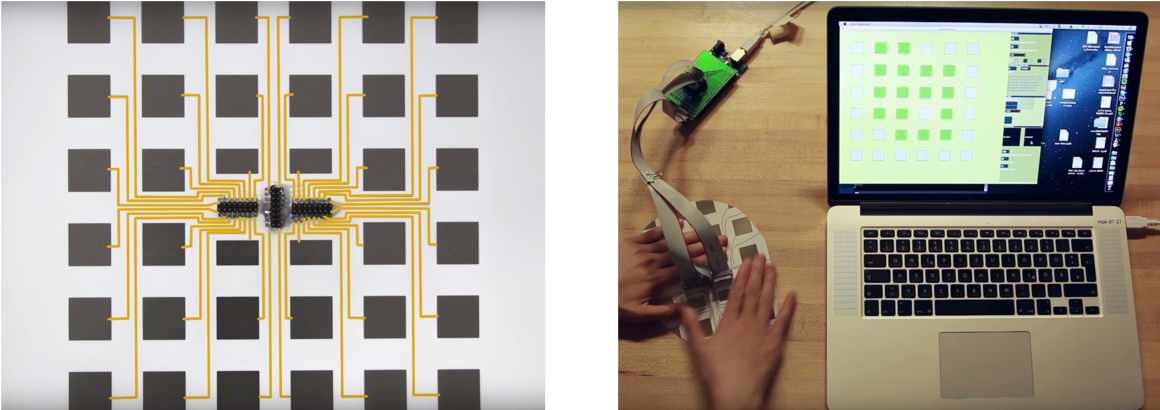
\includegraphics[width=0.88\columnwidth]{figures/cuttable.png}
	\setlength{\belowcaptionskip}{-6pt}
    \caption{A cuttable multitouch sensor using tree topology electrodes and flexible materials.}
    \label{fig:cuttable}
\end{figure}



\section{Capacitive Touch Interaction Sensing beyond Touchscreens}
Capacitive sensing was introduced into the field of HCI over two decades ago. Recently, Grosse-Puppendahl and his colleagues reviewed and summarized past researches related to capacitive sensing theories and techniques ~\cite{Grosse-Puppendahl-capacitive}. Among all the capacitive sensing methods, shunt mode sensing is the most widely spread approach in implementing modern capacitive touchscreens. The touch panel consists of multiple layers above the display screen with all the sensing nodes oriented in a row-column matrix (Fig ~\ref{fig:multi-layer-touchscreen}). Each node is a high-resolution continuous capacitance measurement sensor. Obtaining the low-level capacitive data from the touchscreen provides us with more capability beyond binary finger touch sensing. 

\begin{figure}[ht]
    \centering
	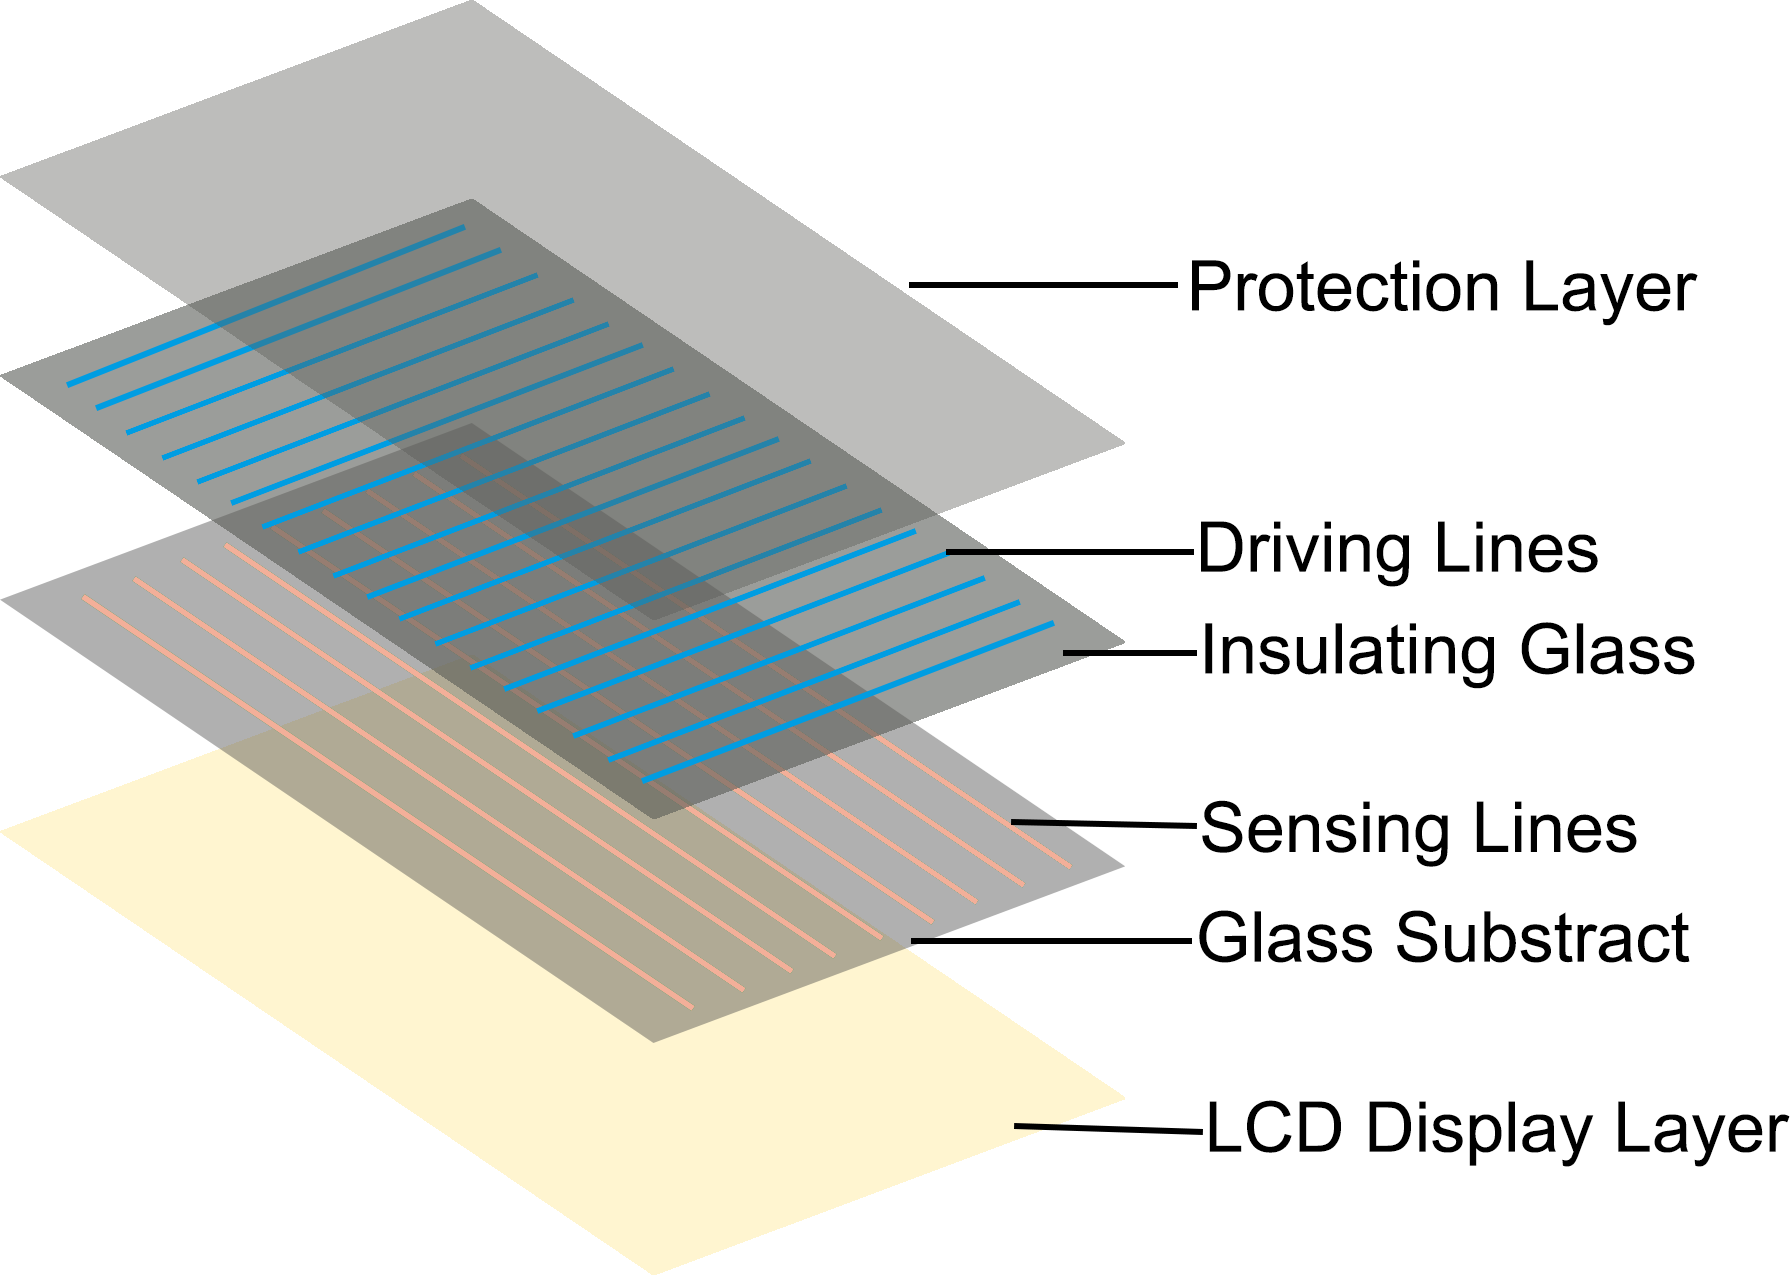
\includegraphics[width=0.78\columnwidth]{figures/multi-layer-touchscreen.png}
	\setlength{\belowcaptionskip}{-6pt}
    \caption{The multi-layer structure of mutual capacitance touchscreen. }
    \label{fig:multi-layer-touchscreen}
\end{figure}

Similar to our approach, \textit{BodyPrint} ~\cite{Holz-bodyprint} and \textit{CapAuth} ~\cite{Guo2015} (Fig ~\ref{fig:capacitive-auth}) combined capacitive touchscreens with machine learning classifiers to provide authentication and even identification of users by recognizing different patterns of capacitance image on touchscreen. \textit{PalmTouch} enabled the palm as an additional input modality to enhance mobile interaction ~\cite{Le-palmtouch}. Researchers also explored the potential of using the raw capacitive data of touchscreens to support sensing of tangible 3D-printed gadgets on top of the screen ~\cite{Chan-CapStones, Schmitz2017, Schmitz2018}. While these prior works share the same raw capacitance signal as our approach, we focus on fabricating conductive interfaces to support large-scale, flexible touch interfaces on the ambient surfaces connected to touchscreens.

\begin{figure}[ht]
    \centering
	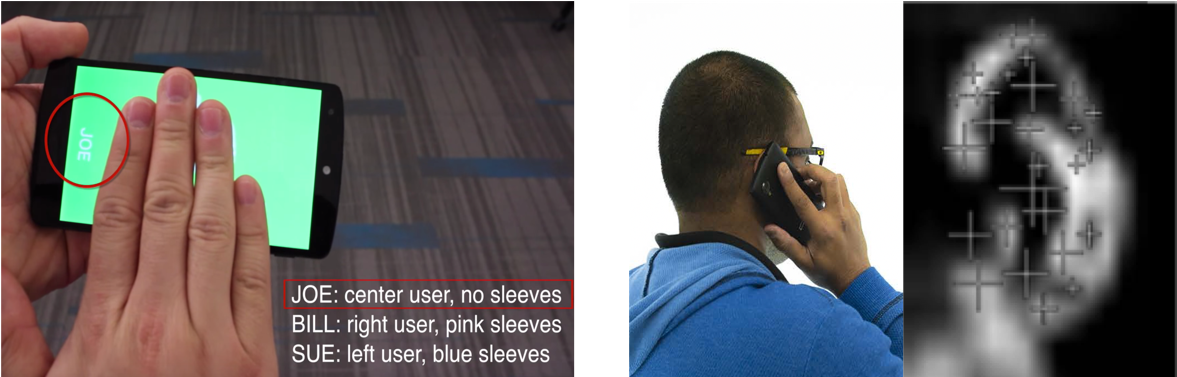
\includegraphics[width=0.88\columnwidth]{figures/capacitive-auth.png}
	\setlength{\belowcaptionskip}{-6pt}
    \caption{User authentications using capacitive sensors on touchscreen.}
    \label{fig:capacitive-auth}
\end{figure}

Modern mobile devices are embedded with rich sensors and actuators. Researchers have explored approaches and techniques enhancing the interaction around mobile devices with customized sensors via active and passive techniques. Researchers have explored attaching capacitive sensors to mobile devices to enable interactive user applications. iGrasp ~\cite{Cheng2013a} and IrotateGrasp ~\cite{Cheng-2013-IrotateGrasp} used capacitive touch sensors on the edge and back of the mobile device to recognize the hold postures for adaptive keyboard layout and screen rotation. These approaches demonstrate promising applications space, however, the requirement of external sensors, power source and processing unit create barriers for massive adoption.

Researchers also explored leveraging the built-in sensors to enhance the interaction on or around the touchscreen. Acoustruments ~\cite{laput2015acoustruments} constructed various sensing units that can detect hand interaction around mobile devices such as touch, proximity and rotation by measuring the acoustic signal transmitted in an enclosed, pipe-like pathway from the speaker to the microphone. UbiTouch ~\cite{wen2016ubitouch} enabled touch interface on surrounding surfaces using build-in proximity and ambient light sensors. Wang and colleagues presented a virtual keyboard technique on the surrounding surface of mobile devices through harnessing multipath fading with multiple built-in microphones ~\cite{wang2014ubiquitous}. 

In close proximity to our work, researchers explored methods extending touch interaction from the touchscreen to ambient objects or surfaces with conductive materials. \textit{Clip-on Gadgets} extended capacitive touchpoints on the phone to physical controllers via conductive materials ~\cite{Yu2011}. Kato and his colleagues went a step further, fabricating 3D-printed conductive gadgets with haptic feedback patterns ~\cite{Kato2016}. User interaction with these gadgets was detected via the capacitive screen when they were placed onto the phone. In addition, they also presented a technique named \textit{ExtensionSticker} which allowed touch sensing to be transferred to ambient surfaces ~\cite{Kato2015, Kato2015a}. However, without accessing the raw capacitive data, \textit{ExtensionSticker} could not support large-scale touch interfaces. Long-range conductive strips attached on touchscreens would be recognized by the built-in touch detector as finger touch events, which prevents the detection of real touches on the strip. As a result, these extension-sticker techniques only allow for near-range touch sensing interfaces. Recently, Gao and Ikematsu demonstrated the feasibility of using 1D conductive ink strips or ABS filament arrays sensing 2D finger positioning ~\cite{mobicom-gao18, Ikematsu-Ohmic-Touch} through measuring the resistance introduced to the touchscreen's sensing circuit. However, they only demonstrated short-range applications such as 2D finger tracking on phone-based VR headsets or 1D touch bar using a single sensor node. Though these work already provides diverse interaction surrounding smartphone, they are not able to differentiate off-screen touch and on-screen touch. In some cases when user is conducting on-screen touch, it is possible for the smart device to mistakenly recognize the event as off-screen touch due to the similarity of capacitive image pattern.

\begin{figure}[ht]
    \centering
	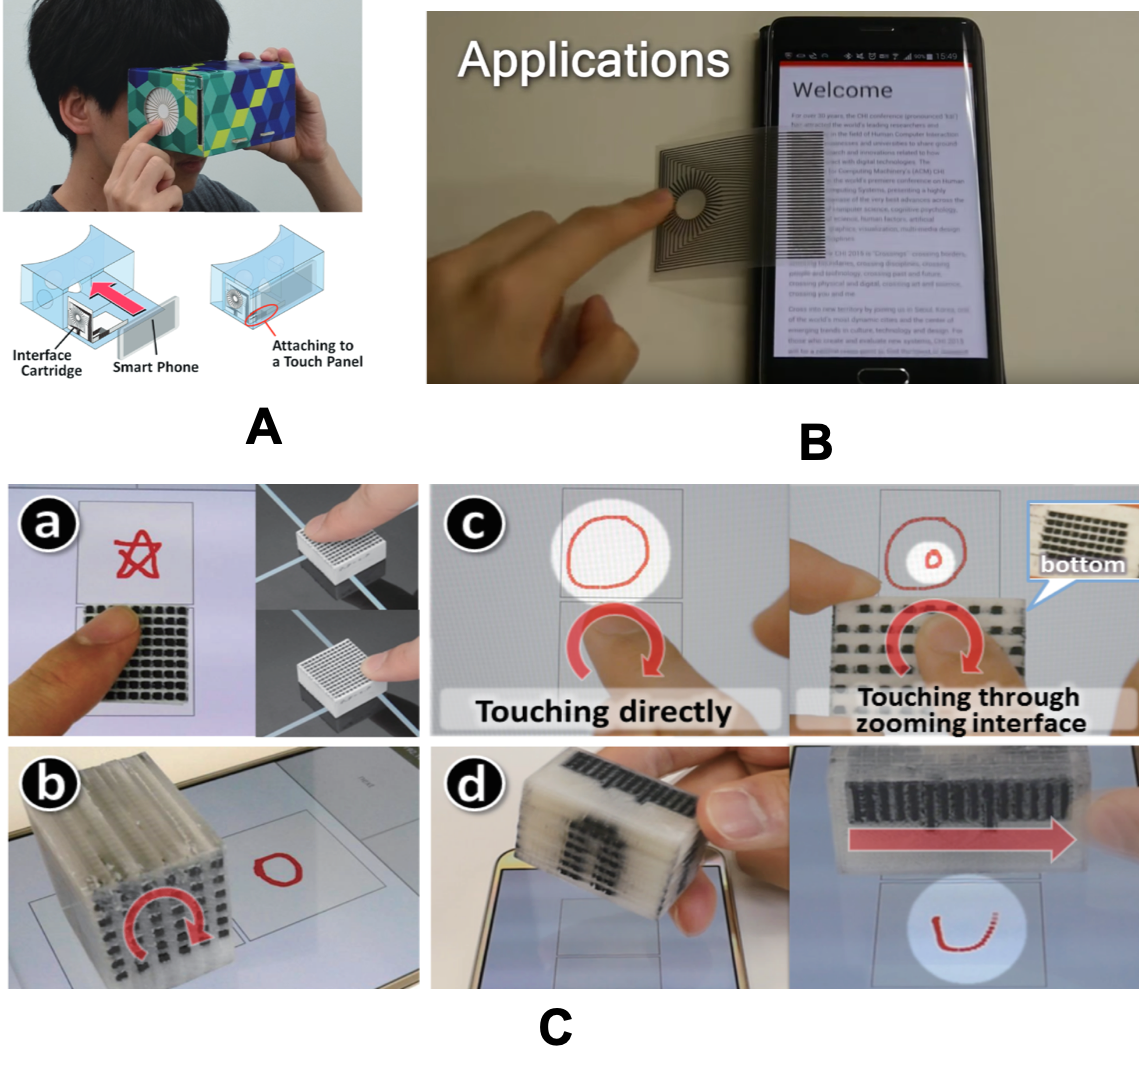
\includegraphics[width=0.88\columnwidth]{figures/ambient-capcitive-sensing.png}
	\setlength{\belowcaptionskip}{-6pt}
    \caption{Extending touch interaction to ambient objects using strip-like conductive materials. A: Mobile head-mounted display with proprietary controller. B: Smartphone side-input controller. C: Conductive gadget that enables touching, zooming and sliding interaction.}
    \label{fig:ambient-capcitive-sensing}
\end{figure}

In contrast with prior work, \textit{FlexTouch} can perfectly differentiate on-screen touch from off-screen touch based on our study of raw capacitance signal of these two interaction modes. More importantly, \textit{FlexTouch} allows users to create large-scale, passive, flexible and customizable touch sensitive gadgets that can be easily attached to the mobile touchscreen for rapid prototyping of interactive applications. To further empower large-scale capacitive sensing, we leverage the local ground plane of the touchscreen to boost capacitance signal strength that enables touch-sensing coverage range up to 4 meters and objects' presence sensing range up to 2 meters, which we think is a significant milestone in large-scale touchscreen-based capacitive sensing. This capability allows \textit{FlexTouch} to support large-scale sensing applications such as touch sensitive yoga mats or bed mattresses with signal processing and machine learning techniques. These advancements provide \textit{FlexTouch} with potentials to be applicable to a variety of new touch sensing applications beyond prior works.

\section{Summary}
In this chapter, we walked through the body of literature related to our work, and introduced several different touch sensing techniques, ranging from acoustic sensing, electromagnetic sensing to capacitive sensing, that are applied to augment the interactivity of everyday surfaces and objects. Some work already supports large-scale touch sensing, but dedicated sensing platform and external power are essential to these systems. Then we took a closer look at capacitive sensing beyond touchscreens. We introduced some work that innovatively leverage the embedded sensors in smartphone for user authentications. Coupled with smartphone, well-designed touch interface like \textit{ExtentionSticker} and conductive gadget make full use of touchscreen that provide user with a more natural and efficient way of basic interactions around smartphone. However, these interactions are only augmentation or a form of translation of on-screen touch, which heavily relies on existing touch events such as click, and does not allow user to define customizable off-screen interaction. Finally, we introduced our work \textit{FlexTouch}, which specifically solve the off-screen detection problem as well as interaction scaling problem.